\section{Design}
\label{sec:Design}

\subsection{Architecture Design}
\label{sec:Design>Architecture Design}
Because we selected the web application model from the beginning, the classic client-server web architecture was quickly adopted. The architecture is a distributed application structure that partitions tasks or workloads between the providers of a resource or service, called servers, and service requests called clients. In theory, any device connected to the Internet can try to access and obtain the resources or services of the server while the server is running normally. Based on the client-server structure, we have detailed its component structures below:

\subsubsection{Web Browser or Client}
\label{sec:Design>Architecture Design>Web Browser or Client}
The web browser or client is the interface rendition of a web app functionality, with which the user interacts. This content delivered to the client is developed using HTML, JavaScript, and CSS and does not require operating system related adaptations. In essence, the web browser or client manages how end users interact with the application.

There are three, well-known Web Application Architecture types available in the modern landscape: Single Page Applications (SPA), Microservices, and Serverless Architectures. Because the SPA is super-simple to deploy if compared to more traditional server-side rendered applications: it is just one index.html file, with a CSS bundle and a Javascript bundle. Furthermore, our frontend and backend are developed separately. We chose the SPA structure.

The SPA model interacts with the user by providing updated content within the current page rather than loading entirely new pages from the server with each action from the user. It helps prevent interruptions in the user experience, transforming the behavior of the application such that it resembles a traditional desktop application.

\subsubsection{Web Application Server}
\label{sec:Design>Architecture Design>Web Application Server}
The web application server manages business logic and data persistence and can be built using PHP, Python, Java, Ruby, .NET, Node.js, among other languages. It is comprised of at least a centralized hub or control center to support multi-layer applications. The essential purpose of a web server architecture is to complete requests made by clients for a website. The clients are typically browsers and mobile apps that make requests using secure HTTPs protocol, either for page resources or a REST API.

Since the focus of this project is on the client side (frontend), which is the map generator (written in JavaScript), we chose the Node.js. Moreover, the Node.js is written using JavaScript and is the same technology as frontend components. This makes it easier for the developer to program backend services and frontend user interfaces. It also provides consistency, code sharing and reusability, simple knowledge-transfer, and a large number of free tools. These benefits bring flexibility and efficiency when building this project.

\subsubsection{Database Server}
\label{sec:Design>Architecture Design>Database Server}
The database server provides and stores relevant data for the application. Additionally, it may also supply the business logic and other information that is managed by the web application server. There are multiple popular database systems available: Oracle, MySQL, Microsoft SQL Server, PostgreSQL, MongoDB, MariaDB, DB2, and SAP HANA.

Because the project involves a small number of entities, the relationships among entities are not complicated, and the choice of the Software Development Life Cycle (SDLC) model, we chose the MongoDB, which is dynamic, flexible and easy to get started. It also provides high performance, high availability, and high scalability. More importantly, our main purpose is to save maps and implement basic CRUD (create, retrieve, update, delete) operations of the database. As MongoDB is a schema-less database (written in C++), we can serialize the map data to JSON, send it to MongoDB and then save it.

\subsection{Database Design}
\label{sec:Design>Database Design}
NoSQL stands for "not only SQL," which is an approach to database design that can accommodate a wide variety of data models, including key-value, document, columnar and graph formats. MongoDB is a type of NoSQL database. A record in MongoDB is a document, which is a data structure composed of field and value pairs. MongoDB documents are similar to JSON objects, because the values of fields may include other documents, arrays, and arrays of documents.

The system supports only two document types: the user and the map. A user can have many maps, but a map can only belong to one user. Thus, the relationship between the user and the map should be one-to-many.

MongoDB provides two ways of data modeling: Embedded Data Modeling and Normalized Data Modeling. Using Embedded Data Modeling, we may embed related data in a single structure or document, which means we should store maps in the user schema. However, the data of the map is relatively large, in general, it may exceed the maximum BSON document size set by the MongoDB, and the map cannot exist as a separate entity. Though embedding provides better performance for reading operations, as well as the ability to request and retrieve related data in a single database operation, it is still beyond our consideration.

Normalized Data Modeling provides One-to-One and One-to-Many Relationships. We chose the Normalized One-to-Many Structure, which uses references between documents, and provides more flexibility than embedding. Figure \ref{fig:ER Diagram} is the Entity Relationship Diagram that describes the relationship between the user and the map.

\begin{figure}[htbp]
\centering
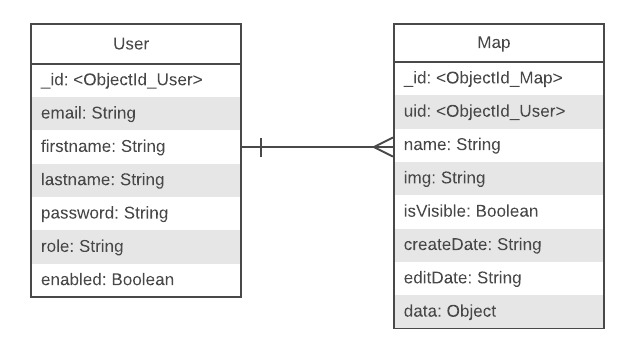
\includegraphics[width=\textwidth]{section03/assets/ER_Diagram.png}
\caption[Entity Relationship Diagram]{\label{fig:ER Diagram}Entity Relationship Diagram}
\end{figure}

\subsection{REST API Design}
\label{sec:Design>REST API Design}
REST is the acronym for Representational State Transfer. It is an architectural style for distributed hypermedia systems and was first presented by Roy Fielding in 2000 in his famous dissertation \cite{Fielding00architecturalstyles}.

Like any other architectural styles, REST has its own 6 guiding constraints, which must be satisfied if an interface conforms to the RESTful. These principles are listed below:
\begin{enumerate}
  \item Client–server. By separating the user interface concerns from the data storage concerns, it improves the portability of the user interface across multiple platforms and improve scalability by simplifying the server components.
  \item Stateless. Each request from a client to server must contain all of the information necessary to understand the request, and cannot take advantage of any stored context on the server. Session state is therefore kept entirely on the client.
  \item Cacheable. Cache constraints require that the data within a response to a request be implicitly or explicitly labeled as cacheable or non-cacheable. If a response is cacheable, then a client cache is given the right to reuse that response data for later, equivalent requests.
  \item Uniform interface. By applying the software engineering principle of generality to the component interface, the overall system architecture is simplified, and the visibility of interactions is improved.
  \item Layered system. The layered system style allows an architecture to be composed of hierarchical layers by constraining component behavior such that each component cannot ``see'' beyond the immediate layer with which they are interacting.
  \item Code on demand (optional). REST allows client functionality to be extended by downloading and executing code in the form of applets or scripts.
\end{enumerate}

Based on these principles, we have designed the APIs shown in Table \ref{tab:REST API Design Table}.
\begin{table}[!htb]
  \centering
  \begin{tabularx}{\textwidth}{>{\raggedright}cXX}
    \toprule[1.5pt]
    \textbf{HTTP Verb} & \textbf{URI} & \textbf{Description}
    \\ \midrule[1.5pt]
    % POST & /metro/auth/signup & Sign up for a new account
    % \\ \midrule
    % POST & /metro/auth/login & Log in to the system
    % \\ \midrule
    % POST & /metro/auth/logout & Log out of the system
    % \\ \midrule
    GET & /metro/api/v1/users & Get a list of all users
    \\ \midrule
    GET & /metro/api/v1/users/\{uid\} & Get the user with \{uid\}
    \\ \midrule
    GET & /metro/api/v1/users/\{uid\}/ maps & Get a list of all maps of the user with \{uid\}
    \\ \midrule
    PATCH & /metro/api/v1/users/\{uid\}/ password & Verify the password of the user with \{uid\}
    \\ \midrule
    PUT & /metro/api/v1/users/\{uid\}/ password & Update the password of the user with \{uid\}
    \\ \midrule
    PUT & /metro/api/v1/users/\{uid\}/ email & Update the email of the user with \{id\} \\ \midrule
    PUT & /metro/api/v1/users/\{uid\}/ name & Update the name of the user with \{id\} \\ \midrule
    PUT & /metro/api/v1/users/\{uid\}/ enabled & Update the enabled of the user with \{uid\}
    \\ \midrule
    GET & /metro/api/v1/maps/\{mid\} & Get the map with \{mid\}
    \\ \midrule
    GET & /metro/api/v1/maps/ ?page=\{page\}\&limit=\{limit\} & Get a list of \{limit\} maps on page \{page\}
    \\ \midrule
    POST & /metro/api/v1/maps & Add a new map to the database
    \\ \midrule
    PUT & /metro/api/v1/maps/\{mid\} & Update the map with \{mid\}
    \\ \midrule
    DELETE & /metro/api/v1/maps/\{mid\} & Delete the map with \{mid\}
    \\ \bottomrule[1.5pt]
  \end{tabularx}
  \caption[REST API Design Table]{REST API Design Table}
  \label{tab:REST API Design Table}
\end{table}

\subsection{Map Generator Design}
\label{sec:Design>Map Generator Design}
\subsubsection{Canvas and SVG}
\label{sec:Design>Map Generator Design>Canvas and SVG}
Since the project is a web application, the map generator should run on the web page. We need to choose a 2D HTML Graphics Tool to render it, such as Canvas or SVG.

SVG is a language for describing 2D graphics in XML, which means every element is available within the SVG DOM, you can attach JavaScript event handlers for an element. In SVG, each drawn shape is remembered as an object. If attributes of an SVG object are changed, the browser can automatically re-render the shape. Canvas draws 2D graphics, on the fly (with a JavaScript) by rendering pixel by pixel. In canvas, once the graphics are drawn, it is forgotten by the browser. If its position should be changed, the entire scene needs to be redrawn, including any objects that might have been covered by the graphics. We chose Canvas not only because there are always many elements in a map, but also there are many third-party JavaScript graphics libraries that can provide support.

\subsubsection{Graphics Libraries}
\label{sec:Design>Map Generator Design>Graphics Libraries}
The more important thing is that we have not had any experience in developing a map generator before. However, we learned the necessary knowledge to maintain the continuation of development from similar websites, which mentioned in the section Background. In addition, developing this generator requires much professional geometric mathematics. If we build our own wheels, the time may not be enough. There are many open source third-party graphics libraries on the web, such as D3.js, Paper.js, Fabric.js, Three.js, and so on, which provide many ready-made and mature geometric construction methods. D3.js was chosen because of the following reasons:
\begin{enumerate}
  \item It is open source: so we can freely use the library, code and build our own maps.
  \item It has good and neat documentation of all the available functions and methods.
  \item There is a gallery with unique charts which can be referred to while developing our project.
\end{enumerate}

\subsubsection{Height Map}
\label{sec:Design>Map Generator Design>Height Map}
Before we get started to develop this map generator, we need to understand what is a map and decide what methods we are going to use to generate it. Simplifying the map is a two-dimensional representation of the surface of the world. The main thing that allows us to say whether an image is a map or not is the obvious partition between land and water parts. To have an ability to divide a canvas into land and water we need to know what pieces are lower than others, it means we need to generate a height map.

There are three main ways to generate a heightmap: use noise functions, use graph structure, or use both. Most procedural map generators use noise functions (midpoint displacement, fractal, diamond-square, Perlin noise, etc.) to generate a height map, but the result may look a bit like artificial. So we decided to use graph structure to model the things directed by gameplay constraints (elevation, affluence, desirability, district, buildings). We want this project to have the following main features:

\begin{enumerate}
  \item Once opening the map editor page, it will show an empty map with random map seeds by default, then the user can start making and editing maps by accessing the menu on the right.
  \item Entering the number of map seeds to create a new empty map in the menu or using the default seeds.
  \item Viewing different types of layers for the map: elevation, affluence, desirability, district, and building, which can superimpose on each other.
  \item Selecting different types of layers for the map: elevation, affluence, desirability, district, and building, which can superimpose on each other.
  \item Displaying street names or not.
  \item Manipulating the ``increase/decrease toggle'' to increase or decrease the value of elevation, affluence, and district.
  \item Manipulating the ``increment sliding'' to set the size of the increment.
  \item Manipulating the ``waterline sliding'' to make map cells as water or city.
  \item If the waterline is changed, the continent will be changed accordingly.
  \item Displaying contour lines or not.
  \item After selecting one or more than one layers under ``edit'' mode, the user can change the size of the "soft brush" by using the mouse wheel, which determines the area where the map will be edited.
  \item Editing the map by clicking and dragging the ``soft brush.''
  \item The districts and buildings are procedurally generated.
  \item Allowing to change the type of the current district by right-clicking and selecting a new type from the context menu.
  \item The map provides 13 different types of districts: rich, medium, poor, empty, plaza, park, farm, water, harbor, university, religious, castle, and military.
  \item Zooming in and zooming out the map by pressing on the alt key and using the mouse wheel.
  \item Using a specialized button to resize the map on the right top.
  \item Saving the map or downloading it by clicking the button on the right bottom.
\end{enumerate}

All these are based on the Voronoi diagram. Thankfully, generating Voronoi diagrams in JavaScript is easy to be implemented if we use d3.voronoi of Fortune’s algorithm by Mike Bostock.
